\documentclass[12pt, a4paper]{report}
\usepackage[top=1cm, left=1cm, right=1cm]{geometry}

\usepackage[utf8]{inputenc}
\usepackage[russian]{babel}

\usepackage{array}
\newcolumntype{M}[1]{>{\centering\arraybackslash}m{#1}}

\usepackage{hyperref}
\hypersetup{
	colorlinks,
	citecolor=black,
	filecolor=black,
	linkcolor=black,
	urlcolor=black
}

\usepackage{sectsty}
\allsectionsfont{\centering}

\usepackage{indentfirst}
\setlength\parindent{24pt}

\usepackage{algorithm}
\usepackage[noend]{algpseudocode}

\usepackage{listings}
\usepackage{xcolor}
\definecolor{codegreen}{rgb}{0,0.6,0}
\definecolor{codegray}{rgb}{0.5,0.5,0.5}
\definecolor{codepurple}{rgb}{0.58,0,0.82}
\definecolor{backcolour}{rgb}{0.95,0.95,0.92}
\lstdefinestyle{mystyle}{
    backgroundcolor=\color{backcolour},
    commentstyle=\color{codegreen},
    keywordstyle=\color{magenta},
    numberstyle=\normalsize\color{codegray},
    stringstyle=\color{codepurple},
    basicstyle=\ttfamily\footnotesize,
    breakatwhitespace=false,
    breaklines=true,
    captionpos=b,
    keepspaces=true,
    numbers=left,
    numbersep=5pt,
    showspaces=false,
    showstringspaces=false,
    showtabs=false,
    tabsize=2
}

\usepackage{graphicx}
\graphicspath{ {plots/pictures/}{assets/pictures} }

\begin{document}
	\begin{titlepage}
		\begin{center}
			\large \textbf{Министерство науки и высшего образования Российской Федерации} \\
			\large \textbf{Федеральное государственное бюджетное образовательное учреждение высшего образования} \\
			\large \textbf{«Российский химико-технологический университет имени Д.И. Менделеева»} \\

			\vspace*{4cm}
			\LARGE \textbf{ОТЧЕТ ПО ЛАБОРАТОРНОЙ РАБОТЕ №9}

			\vspace*{4cm}
			\begin{flushright}
				\Large
				\begin{tabular}{>{\raggedleft\arraybackslash}p{9cm} p{10cm}}
					Выполнил студент группы КС-36: & Золотухин А.А. \\
					Ссылка на репозиторий: & https://github.com/ \\
					& MUCTR-IKT-CPP/ \\
					& ZolotukhinAA\_36\_ALG \\
					Принял: & Крашенников Роман Сергеевич \\
					Дата сдачи: & 05.05.2025 \\
				\end{tabular}
			\end{flushright}

			\vspace*{6cm}
			\Large \textbf{Москва \\ 2025}
		\end{center}
	\end{titlepage}

	\tableofcontents
	\thispagestyle{empty}
	\newpage

	\pagenumbering{arabic}

	\section*{Описание задачи}
	\addcontentsline{toc}{section}{Описание задачи}
	\large
	В рамках лабораторной работы необходимо реализовать алгоритм хэширования: \textit{SHA1}. \par
	Дополнительный вариант: \textit{Luffa}, \textit{SHA3}. \par
	Для реализованной хеш-функции провести следующие тесты:
	\begin{itemize}
		\item провести сгенерировать \underline{1000} пар строк длинной \underline{128} символов отличающихся друг от друга \underline{1},\underline{2},\underline{4},\underline{8},\underline{16} символов и сравнить хеши для пар между собой, проведя поиск одинаковых последовательностей символов в хешах и подсчитав максимальную длину такой последовательности. Результаты для каждого количества отличий нанести на график, где по оси \textit{х} кол-во отличий, а по оси y максимальная длинна одинаковой последовательности;
		\item провести $N = 10^{i}$(i от 2 до 6) генерацию хешей для случайно сгенерированных строк длинно 256 символов, и выполнить поиск одинаковых хешей в итоговом наборе данных, результаты привести в таблице, где первая колонка это \textit{N} генераций, а вторая таблица наличие и кол-во одинаковых хешей, если такие были;
		\item провести по \underline{1000} генераций хеша для строк длинной n (\underline{64}, \underline{128}, \underline{256},\underline{ 512}, \underline{1024}, \underline{2048}, \underline{4096}, \underline{8192})(строки генерировать случайно для каждой серии), подсчитать среднее время и построить зависимость скорости расчета хеша от размера входных данных.
	\end{itemize}

	\newpage

	\section*{Описание метода/модели}
	\addcontentsline{toc}{section}{Описание метода/модели}
	\large
	\textbf{Хеш-функция} - структура данных, реализующая интерфейс ассоциативного массива. \par
	Для такой таблицы значений, как правило, реализуются следующие операции:
	\begin{itemize}
		\item \textbf{Вставка(k, v)} - вставить в таблицу элемент с ключом;
		\item \textbf{Удаление(k)} - удалить из таблицы элемент с ключом;
		\item \textbf{Поиск(k)} - найти в таблице элемент с ключом;
	\end{itemize}
	При этом выделяется \underline{2} вида таких таблиц:
	\begin{itemize}
		\item \textbf{Set} - таблица, хранящая в себе множество значений, каждое из которых само по себе является ключом и значением одновременно;
		\item \textbf{Map} - таблица, хранящая в себе пары ключ-значение в явном виде.
	\end{itemize}

	\textbf{Хэширование} - применение особого алгоритма к некоторым входным данным произвольного типа, преобразующего их в битовую строку установленной длины, строка часто выводится в форме шестнадцатеричного числа. \par
	Алгоритм, который применяется для хеширования, называют \textbf{хеш-функцией}. \par
	Результат работы алгоритма хеширования называют \textbf{хешем} \par
	\textbf{Криптографическая хеш-функция} - это специальный класс хеш-функций, который имеет различные свойства, необходимые для криптографии. \par
	\textbf{Лавинный эффект} - ситуация, в которой при генерации хеша для двух слабо отличающихся друг от друга изначальных набора данных, результат будет отличаться колоссально. \par
	\textbf{Соль} - дополнительные данные, которые вносятся в хеш-функцию и генерируются случайным образом. \par
	Соль может быть:
	\begin{itemize}
		\item \textit{Статическая} - одинаковая на каждый хеш;
		\item \textit{Динамическая} - разная для каждого хеша.
	\end{itemize}

	\textbf{SHA-1} - Secure Hash Algorithm 1 (1995). Использует 160 бит для хранения результата. \par
	\textbf{SHA-3} - Secure Hash Algorithm 3. \par
	Исходное сообщение разбивается на блоки по 512 бит в каждом. Последний блок дополняется до длины, кратной 512 бит. Сначала добавляется 1 (бит), а потом — нули, чтобы длина блока стала равной 512 — 64 = 448 бит. В оставшиеся 64 бита записывается длина исходного сообщения в битах (в big-endian формате). Если последний блок имеет длину более 447, но менее 512 бит, то дополнение выполняется следующим образом: сначала добавляется 1 (бит), затем — нули вплоть до конца 512-битного блока; после этого создается ещё один 512-битный блок, который заполняется вплоть до 448 бит нулями, после чего в оставшиеся 64 бита записывается длина исходного сообщения в битах (в big-endian формате). Дополнение последнего блока осуществляется всегда, даже если сообщение уже имеет нужную длину.

	\newpage

	\section*{Выполнение задачи}
	\addcontentsline{toc}{section}{Выполнение задачи}
	SHA-1 реализован на языке \textit{Java}. Построение графиков проводились с помощью программы \textit{GNUplot}.

	\newpage
	\vfill

	\begin{figure}[h]
		\centering
		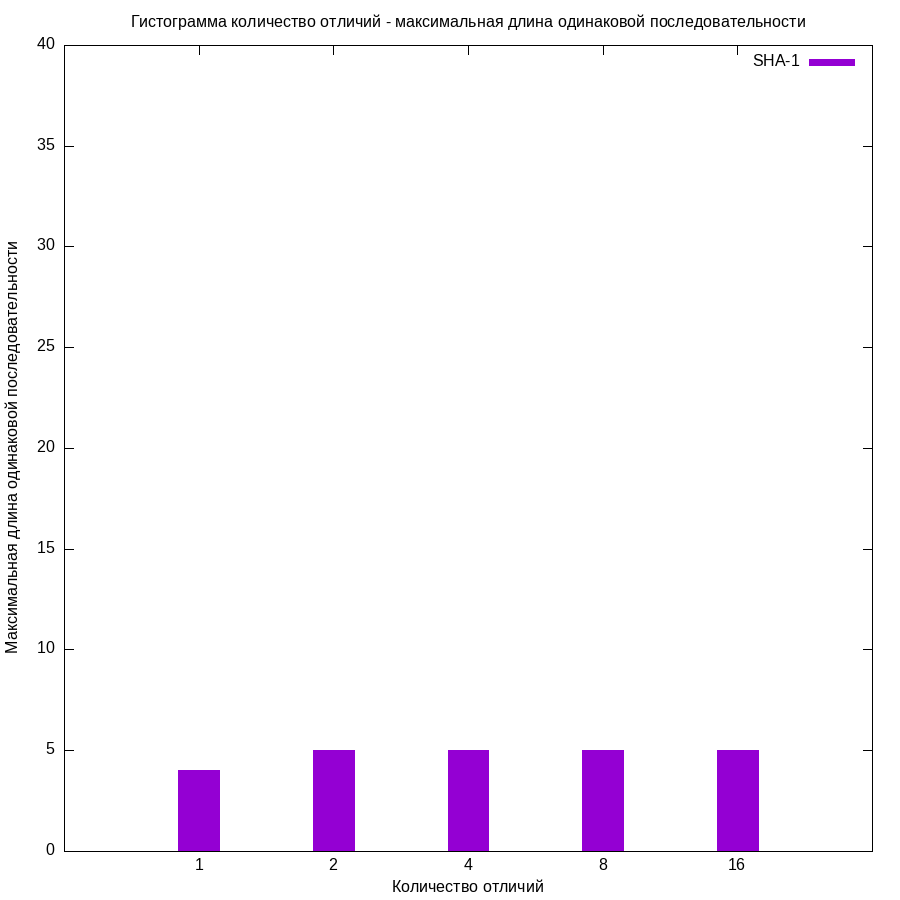
\includegraphics[width=200pt]{sha1_similarity.png}
		\caption{Гистограмма количество отличий - максимальная длина одинаковой последовательности}
	\end{figure}

	\begin{figure}[h]
		\centering
		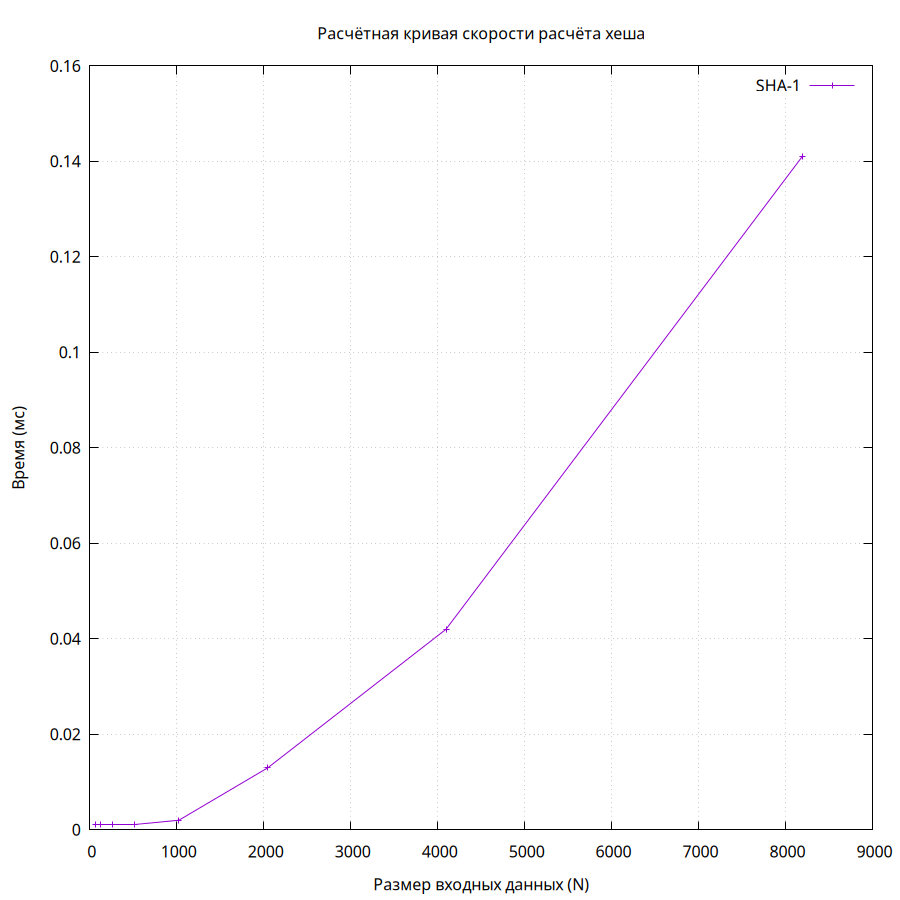
\includegraphics[width=200pt]{sha1_speed.png}
		\caption{Расчётная кривая скорости расчёта хеша.}
	\end{figure}

\end{document}
